\chapter{Evaluation}\label{sec:evaluation}


% \begin{blockquote}
%     \paragraph{Intent:} Performance evaluation 
%     Structure:
%     \begin{description}

%         \item[Experimental setup] Optimization problems types, evaluation assumption and budget, repetition

%         \item[Benhmark 1] Default Tutor-model(portfolio, thresholds) on plethora types of multiobjective problems
%         \begin{enumerate}
%             \item default Tutor-model parameters
%             \item surrogate portfolio items
%             \item Baseline: MOEA
%         \end{enumerate}

%         \item[Benhmark 2] Parameter selection of Tutor-model with the dynamic sampling plan
%         \begin{enumerate}
%             \item Parameters: prediction count, train/test split, stacking solutions. thresholds(x2), solver
%             \item Subset of problems
%             \item Baseline: Static vs Dynamic. Parameters tune
%         \end{enumerate} 

%         \item[Benhmark 3] Many-objective optimization. Objectives>10
%         \begin{enumerate}
%             \item Static Heterogeneous compositional surrogate vs. Homogeneous compositional surrogate
%             \item Base line: MOEA or Random
%         \end{enumerate}

%         \item[Discussion] Results interpretation
%     \end{description}
% \end{blockquote}


In this chapter, we demonstrate the advantages of the use of the developed approach with the compositional surrogate over the static compound in surrogate-based optimization.

% ? MOEA is called globally convergent if the produced, non-dominated population converges to the true Pareto front while the number of generations goes to infinity.


% --------------------------------------------------------------------------------------------
% ------------------------------------------------     Experimental setup     
% --------------------------------------------------------------------------------------------
\section{Experimental setup}

    % ---------------------------------     Optimization problems
    \subsection{Optimization problems}
    Numerous types of problems need to be considered to reduce the bias of the results. For comparison was selected several comprehensive synthetic benchmark suites. All of them are scalable in parameters space and some are scalable in objective space. The problems are designed so that a meaningful comparison can be obtained for optimization techniques. In all cases, a global minimum is expected.

    The following property \cite{WFGref} could characterize the optimization problems:
    \begin{itemize}
        \item \emph{Modality} is the property of the objectives surface. Test problems are either unimodal with one global optimum or multimodal with several local optima. Multimodal problems are more complicated than unimodal problems and more similar to real-world issues.
        \item The \emph{geometry} of a Pareto optimal surface can directly influence the performance of the algorithm. Problems could be related to inner metrics of algorithms to estimate the dominance in population.
        \item The \emph{bias} of landscape transformations impacts the search process by biasing the fitness landscape. This property means that uniformly distributed parameters mapping to predisposition area in objective space. This type of problem could be challenging if the bias region is far away from the Pareto-optimal front.
        \item \emph{Many-to-one} fitness mapping means that different parameter vector could produce the same objective vector. This property made the search more difficult to optimizers because increase likelihood of that parameters variations do not generate new objective vector.
        \item \emph{Not separability }is a characteristic of the dependence between parameters when the multi-objective problem is not intended to be optimized step-by-step for each objective. Finding optimal points for a separable problem tends to be simpler than for an otherwise similar nonseparable problem.
    \end{itemize}

    % ! [===    Many-to-one, bias, Modality, geometry  ===]
        % -----------------------------  ZDT      
        \paragraph{ZDT} widespread test suite\cite{ZitzlerDT00} was conceived for two-objective problems and took its name from its authors Zitzler, Deb and Thiele. In their paper the authors propose a set of 6 different scalable problems all originating from a well thought combination of functions allowing, by construction, to measure the distance of any point to the Pareto front. Each test function involves a particular feature that is known to cause difficulty in the evolutionary optimization process, mainly in converging to the Pareto-optimal front.
        For the evaluations selected following problems:
        \begin{itemize}
            \item ZDT1 has a convex Pareto-optimal front
            \item ZDT2 has a non-convex Pareto-optimal front
            \item ZDT3 adds a discreteness feature to the front. Its Pareto-optimal front consists of several noncontiguous convex parts. The introduction of a sine function in this objective function causes discontinuities in the Pareto-optimal front, but not in the parameter space.
            \item ZDT4 has 21 local Pareto-optimal fronts and therefore is highly multi-modal. Also called \textit{multifrontal} problems.
            \item ZDT6 has a non-uniform search space: the Pareto-optimal solutions are non-uniformly distributed along the global Pareto front, and also the density of the solutions is lowest near the Pareto optimal front and highest away from the front
        \end{itemize}


        % -----------------------------   DTLZ
        \paragraph{DTLZ} is extensive test suite took its name from its authors Deb, Thiele, Laumanns and Zitzler. It was conceived for the multi-objective problems with scalable fitness and objective dimensions.  All problems in this test suite are box-constrained continuous n-dimensional multi-objective problems, scalable in fitness dimension. Incidentally, there being multiple global optima is why many of the DTLZ problems are Pareto many-to-one. 
        \begin{itemize}
            \item DTLZ1  is one of the more difficult test problems in this test set. DTLZ1 has flat landscape regions, and the optimal Pareto front lies on a linear hyperplane. 
            \item DTLZ2 is a unimodal problem with the concave Pareto front.
            \item DTLZ3 is a multimodal problem with the concave Pareto front. DTLZ3 supposed to be harder to converge towards the optimal Pareto front than DTLZ2.
            \item DTLZ4 is a unimodal problem with biases to a dense area of solutions.
            \item DTLZ5 has a bias for solutions close to this Pareto-optimal curve. This problem may be easy for an algorithm to solve. Because of its simplicity, it is recommended to use in a higher number of objectives.
            \item DTLZ6 is more challenging version of the DTLZ5 problem with the non-linear distance function $g()$ makes it harder to convergence against the Pareto optimal frontier.
            \item DTLZ7 is a unimodal problem for the first objective and multimodal for the rest of the objectives. This problem has the disconnected Pareto-optimal front, which increases the likelihood that an \gls{ea} could fail to find all optimal regions.
        \end{itemize}

        % ------------------------------    WFG
        \paragraph{WFG} test suite \cite{WFGref} was designed to outperform the functionalities of previously implemented test suites. Essential improvements have been achieved in a major type of problems. Also, problems with dependencies between position and distance-related parameters are included. The WFG test suite was introduced by Simon Huband, Luigi Barone, Lyndon While, and Phil Hingston. 
        The test set includes the following problems:
        \begin{itemize}
            \item WFG1 is a unimodal problem with a convex and mixed Pareto optimal geometry. WFG1 skews the relative significance of different parameters by employing different weights in the weighted sum reduction.
            \item WFG2 is a nonseparable and unimodal problem with a convex and disconnected Pareto optimal geometry.
            \item WFG3 is a non-separable, unimodal problem in all its objective except for the last one, which is multimodal.
            \item WFG4 is a multimodal problem with a concave Pareto optimal geometry. The multimodality of this problem has large "hills" that make it more complicated for optimization.
            \item WFG5 is a separable problem with deceptive landscape and a concave Pareto optimal geometry.
            \item WFG6 is the non-separable and unimodal problem. Its Pareto optimal geometry is concave. The non-separable reduction of this problem makes it more complicated than that of WFG2 and WFG3.
            \item WFG7 is the separable and unimodal problem with a concave Pareto optimal geometry. WFG7 together with the WFG1 are the only problems that are both separable and unimodal.
            \item WFG8 is a non-separable and unimodal problem with a concave Pareto optimal geometry.
            \item WFG9 is a multimodal, deceptive and non-separable problem with a concave Pareto optimal geometry. Similar to WFG6, the non-separable reduction of this problem makes it more complicated than that of WFG2 and WFG3.
        \end{itemize}


    % ---------------------------------     Optimization search
    \subsection{Optimization search}
    In this thesis, we do not assume the distinct parameter tuning for optimization algorithms. By default, all EAs operate with population size equal to 100 while other parameters do not change. Default solver for the surrogates portfolio is selected the genetic control that combines MOEA/D and NSGA2 algorithms. Intuition of why this is a right combination: NSGA2 gave stable results with a proper distribution of points in Pareto-front approximation while MOEA/D have good exploration quality with low generation count. This combination should gain better trade-off in exploration and exploitation.

    %! [ ====   NSGA2 vs MOEA/D  ====]

    % ---------------------------------    Portfolio
    \subsection{Surrogate portfolio}
    The most popular and perspective models were selected for a default surrogate portfolio. All of them have benefits and drawbacks that depends on the particular use case. From multi-objective models, there is \emph{Gaussian Process Regressor} that commonly used in the Bayesian optimization. For this type of model should be specified by the prior's covariance. It is defined by passing a kernel object, the hyperparameters of which are optimized during extrapolations of the samples. The kernel for this benchmark is selected from the GPML\cite{RasmussenN10} and illustrate a complex kernel design. The Gaussian Process Regressor with this kernel was used to extrapolate the $CO_2$ concentration as a function of the time $t$. The kernel consists of several components that calibrate to represent a long term, periodic and medium components. Even though this kernel is from another domain, it does give good extrapolation quality for the regression model. Unfortunately, the build time is significant and grows with samples size and dimensionality.

    Three models were selected for composite surrogates which give $3^{obj}$ possible surrogate combinations: 
    \begin{itemize}
        \item Support Vector Regression (SVR) model with RBF kernel. SVR uses the same principles as the SVM for classification with the main idea is to minimize error and to individualize the hyperplane which maximizes the margin. With a motivation to extend the SVR to non-linear data, the kernel function transforms the data into a higher dimensional feature space that could be linearly separate.
        \item Multi-layer Perceptron regressor (MLPRegressor) with three hidden layers. A neural network is a popular and influential approach to approximate the functions landscape.
        \item Gradient Boosting Regressor that uses an ensemble decision tree regressors to produce a single model. Building process goes iteratively, at each step, a new tree is trained against the negative gradient of the loss function, that improve results in the previous step. This method accurate, and it applies to a variety of domain-problem.
    \end{itemize}
    
    As a result, for bi-objective problems, there are no more than ten possible surrogate hypotheses (including multi-objective Gaussian Process Regressor). All models are built and validated in parallel.  For a benchmark purpose, at each optimization round the surrogate portfolio does not change. 

    % ---------------------------------    Benchmark baseline
    \subsection{Benchmark baseline}
    The developed approach in this thesis (class TutorModel) was compared with Hypermapper 2.0\cite{nardi2019practical} that discussed in related work. This toolbox is focused on multi-objective parameter tuning with various types of parameters. Hypermapper used several randomized decision forests models, one for each objective. The general idea is scaling several surrogate models to single-objective criteria and optimize it as a single-objective problem. Besides, a Bayesian model is used to assist a search in obtaining a valid configuration. Hypermapper was successfully used in autotuning computer vision applications and database optimization. Since the sample size is not specified, we have selected it as the default population size for the MOEA algorithm (100 points).

    NSGA 2 was chosen as the benchmark baseline, as it is one of the most well-known algorithm \cite{RamirezRV19}. It is a suitable reference point to compare other approaches. The results of budget-limited optimization algorithms should be closer to those results obtained from NSGA2 with a much larger budget. Budget means the available number of real function evaluations.

% --------------------------------------------------------------------------------------------
% ---------------------       Benchmark 1: Model-tutor: Portfolio with compositional surrogates 
% --------------------------------------------------------------------------------------------
\section{Benchmark 1: Portfolio with compositional surrogates. Dynamic sampling plan. [RQ1, RQ2]}
    In this benchmark, a developed methodology(TutorM) was compared with related approaches in solving all three sets of problems (ZDT, DTLZ, WFG) for 2 objectives and 2(3) parameters. The TutorM includes all features such as dynamic compositional models, surrogate portfolio and validation.

    The surrogate model can significantly accelerate the ascent to the global optimum. For example, figure \ref{fig:changing_models} demonstrates the stable near-optimal solution with significant economy of resource (300 vs. 1000 function estimates).
    Initially, it could be notest that TutorM considerably outperforms NSGA2 and Hypermapper right from the start of their optimisation process (Fig \ref{fig:zdt6_dist}). Besides to interpreter results more involved, non-dominated size should be analysed. ZDT6 landscape has flat regions with local Pareto-front. Hypermapper gets stuck in some of them as evidenced by the serrated graph (Fig \ref{fig:zdt6_ndf}). The drop occurs when discovering a new point in the other Pareto-optimal front. NSGA2 stagnate and comparable to random search due to the many-to-one parameter and objectives mapping. Solutions from the population do not have enough sparsity in objective space to detect optimal search direction. TutorM identifies global Pareto front straightway and increases Pareto-optimal solutions slowly that alike to solutions from NSGA2 with 100 generations (10k evaluations) (Fig \ref{fig:zdt6_front}).

    % === ZDT6
    \begin{figure}
        \centering
        \begin{subfigure}{\textwidth}
            \begin{subfigure}{0.45\textwidth}
                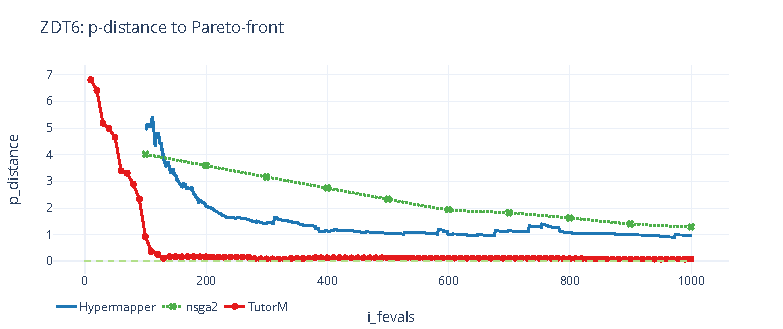
\includegraphics[width=\textwidth]{content/images/zdt6_dist}
                \caption{Average distance of non-dominant solutions to the real Pareto front}
                \label{fig:zdt6_dist}
            \end{subfigure} 
            \begin{subfigure}{0.45\textwidth}
                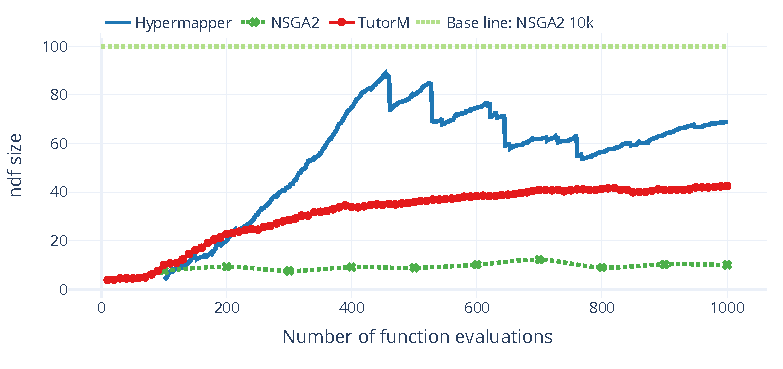
\includegraphics[width=\textwidth]{content/images/zdt6_ndf}
                \caption{Size of non-dominant solutions across the entire set of the measured solutions}
                \label{fig:zdt6_ndf}
            \end{subfigure} 
        \end{subfigure} 

        \begin{subfigure}{\textwidth}
            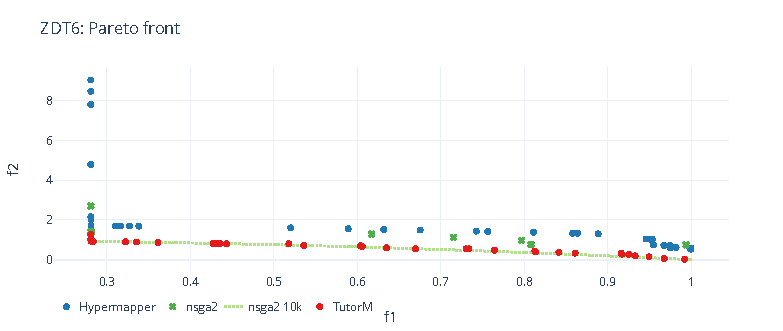
\includegraphics[width=\textwidth]{content/images/zdt6_front}
            \caption{The final assumption of the Pareto optimal solutions (1000 fevals)}
            \label{fig:zdt6_front}
        \end{subfigure} 
        \caption[Comparison of solutions on ZDT6 problem]{A complex comparison of solutions on ZDT6 problem. Final non-dominated points are used to estimate Pareto-optimal solutions.}
        \label{fig:changing_models}    
    \end{figure}


    One of the main advantages of the developed method is the dynamic sampling plan, which depends on the quality of available surrogates. Results show that the number of samples taken from the original plan varies depending on the problem (Figure \ref{fig:changing_models}).
    When samples are enough, several models could periodically swap as best available. It can also be noted that with increasing the sample set, the models give more stable results, and changes become less frequent. In the case of WFG1 problem(\ref{fig:wfg1_models_60}) best accuracy for non-dominated point gave the compositional model with Gradient Boosting Regressor for each objective. In WFG problem, the same compositional model goes ahead other models in the portfolio, but after samples size increased, multi-objective the Gaussian Process Regressor was on the top.
    % === TutorM: surrogate portfolio in action
    \begin{figure}
        \centering
        \begin{subfigure}{\textwidth}
            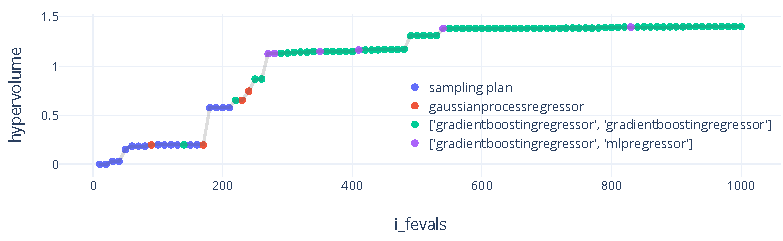
\includegraphics[width=\textwidth]{content/images/dtlz4_models}
            \caption{DTLZ4: sampling plan to the 210th configuration}
            \label{fig:dtlz4_models_210}
        \end{subfigure}
        % \hfill
        
        \begin{subfigure}{\textwidth}
            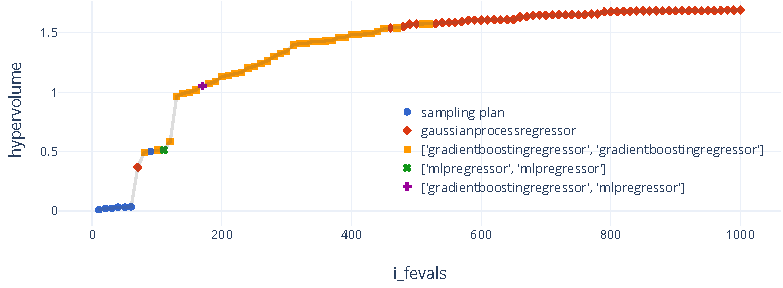
\includegraphics[width=\textwidth]{content/images/wfg1_models}
            \caption{WFG1: sampling plan to the 60th configuration}
            \label{fig:wfg1_models_60}
        \end{subfigure} 

        \caption[Optimization process with dynamic sampling plan and surrogate portfolio.]{Optimization process with dynamic sampling plan and surrogate portfolio. Plots are shown in which step sampling plan was used or which model gives the best accuracy on the test set.}
        \label{fig:changing_models}    
    \end{figure}


    For a satisfactory result, the surrogate model needs to describe the overall landscape and the optimization target area. Figure \ref{fig:wfg_14} shows an example of a case where TutorM produces a better or identical result than an optimal solution. The characteristic of this optimization problem lay in flat landscape regions and relative significance of different parameters that significantly impairs the convergence to the global Pareto-optimal solutions. Hypermapper increase count of non-dominated points, regardless it is local optimum and most samples stack in a small region. NSGA2 after 1000 function evaluations also have high-density regions which could be improved with spending more effort to evaluations. The TutorM found several dozen of Pareto-optimal points, that significantly outperforms Hypermapper and even NSGA2 with 10k evaluations. 
    From WFG4 use case, all over all approaches gain near-optimal results (Fig.\ref{fig:wfg4_front}), but significant advantage over TutorM as it provides an extensive set of solutions (Fig.\ref{fig:wfg4_ndf}) that are well distributed at the Pareto front. As you can see from the graph that the size of the solution increases linearly, which means that effort is spent on improving distribution of the Pareto Pare optimal solutions.


    % As shown in Figure \ref{fig:wfg_14}, TutorM could also outperform the MOEA baseline in 10k evaluations(\ref{sub@fig:wfg1_front}). WFG1 has flat landscape regions hence the convergence of genetic algorithms significantly deteriorates. Hypermapper increase count of non-dominated points, regardless it is local optimum and most samples stack in a small region. Nsga2 after 1000 function evaluations also have high-density regions which could be improved with spending more effort to evaluations. The TutorM has several dozen of Pareto-optimal points from all over the budget, that significantly outperforms Hypermapper and nsga2 even with 10k evaluations. 
    % From WFG4 use case, all over all approaches gain near-optimal results(\ref{fig:wfg4_front}), but significant advantage over TutorM as it provides an extensive set of points(\ref{fig:wfg4_ndf}) that are well distributed at the Pareto front.


    % === WFG1 and WFG4
    \begin{figure}
        \centering
        \begin{subfigure}{\textwidth}
            \begin{subfigure}{0.5\textwidth}
                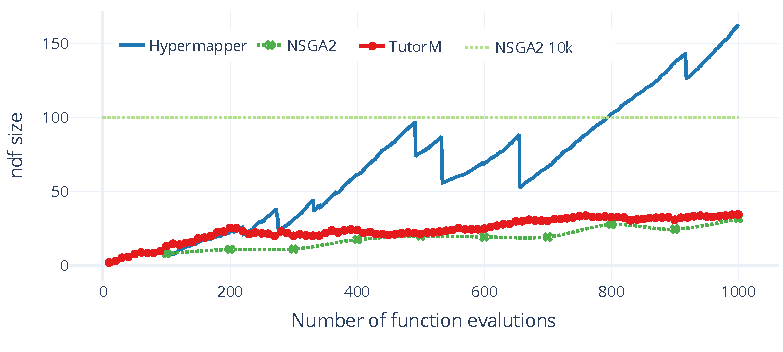
\includegraphics[width=\textwidth]{content/images/wfg1_ndf}
                \caption{WFG1: Size of a non-dominated subset of an evaluated examples}
                \label{fig:wfg1_ndf}
            \end{subfigure} 
            \begin{subfigure}{0.5\textwidth}
                \includegraphics[width=\textwidth]{content/images/wfg1_front}
                \caption{WFG1: Pareto-front approximation}
                \label{fig:wfg1_front}
            \end{subfigure} 
        \end{subfigure} 
        \begin{subfigure}{\textwidth}
            \begin{subfigure}{0.5\textwidth}
                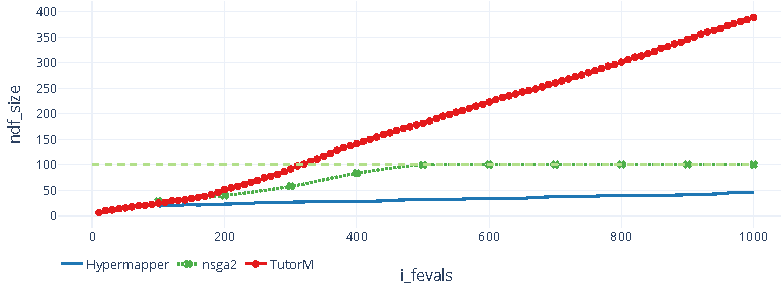
\includegraphics[width=\textwidth]{content/images/wfg4_ndf}
                \caption{WFG4: Size of a non-dominated subset of an evaluated examples}
                \label{fig:wfg4_ndf}
            \end{subfigure} 
            \begin{subfigure}{0.5\textwidth}
                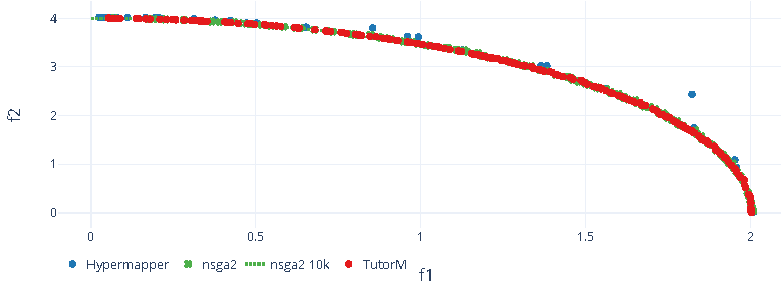
\includegraphics[width=\textwidth]{content/images/wfg4_front}
                \caption{WFG4: Pareto-front approximation}
                \label{fig:wfg4_front}
            \end{subfigure}
        \end{subfigure} 
        \caption[Comparison of solutions on ZDT6 problem]{A complex comparison of solutions on ZDT6 problem. Final non-dominated points are used to estimate Pareto-optimal solutions.}
        \label{fig:wfg_14}    
    \end{figure}


    In this benchmark, we checked all 21 problems from 3 datasets. We considered them as bi-objective with two or three parameters. In all cases, TutorM is ahead of Nypermapper 2.0, and in most cases, TutorM is nearing the baseline solution from NSGA2 with 10k evaluations. The table \ref{tab:magic_five} shows some solutions to the 5 problems. The full list of results is provided in the appendix.
 
        % Please add the following required packages to your document preamble:
    % \usepackage{booktabs}
    % \usepackage{multirow}
    \begin{table}[]
        \centering
        \caption{Comparison of final results after 1000 function evaluations}
        \begin{tabular}{@{}lllllll@{}}
        \toprule
                                                                                                & Metric        & ZDT4             & ZDT6             & DTLZ4             & WFG1             & WFG4             \\ \midrule
        \multirow{4}{*}{\textbf{TutorM}}                                                          & Hypervolume   & \textbf{99,80\%} & \textbf{99,43\%} & \textbf{99,829\%} & \textbf{95,75\%} & \textbf{99,28\%} \\ \cmidrule(l){2-7} 
                                                                                                & p-distance    & \textbf{0,01}    & \textbf{0,09}    & \textbf{0,001}    & -                & -                \\ \cmidrule(l){2-7} 
                                                                                                & ndf-size      & \textbf{50,0\%}  & 4,26\%           & 0,2\%             & 3,44\%           & \textbf{38,90\%} \\ \cmidrule(l){2-7} 
                                                                                                & space-metric  & \textbf{0,78}    & 0,17             & 0,666             & 0,51             & \textbf{1}       \\ \midrule
        \multirow{4}{*}{\textbf{NSGA2}}                                                           & Hypervolume   & 83,43\%          & 83,84\%          & 87,807\%          & 30,52\%          & 83,95\%          \\ \cmidrule(l){2-7} 
                                                                                                & p-distance    & 0,04             & 1,29             & 0,002             & -                & -                \\ \cmidrule(l){2-7} 
                                                                                                & ndf-size      & 8,77\%           & 1,01\%           & 9,600\%           & 3,18\%           & 10\%             \\ \cmidrule(l){2-7} 
                                                                                                & space-metric  & 0,19             & 0,04             & 0,323             & 0,28             & 0,58             \\ \midrule
        \multirow{4}{*}{\textbf{Hypermaper}}                                                      & Hypervolume   & 97,32\%          & 82,86\%          & 64,57\%           & 44,12\%          & 84,39\%          \\ \cmidrule(l){2-7} 
                                                                                                & p-distance    & 0,90             & 1,12             & 0,059             & -                & -                \\ \cmidrule(l){2-7} 
                                                                                                & ndf-size      & 5,42\%           & \textbf{6,25\%}  & 1,177\%           & \textbf{10,24\%} & 3,26\%           \\ \cmidrule(l){2-7} 
                                                                                                & space-metrics & 0,11             & 0,08             & 0,029             & 0,31             & 0,06             \\ \midrule
        \multirow{4}{*}{\textbf{\begin{tabular}[c]{@{}l@{}}NSGA2 50k\\ (Base line)\end{tabular}}} & Hypervolume   & 100\%            & 100\%            & 100\%             & 100\%            & 100\%            \\ \cmidrule(l){2-7} 
                                                                                                & p-distance    & 2,04e-05         & 0,0003           & 8,81e-06          & -                & -                \\ \cmidrule(l){2-7} 
                                                                                                & ndf-size      & 0,72\%           & 0,72\%           & 0,360\%           & 0,72\%           & 0,72\%           \\ \cmidrule(l){2-7} 
                                                                                                & space-metric  & 1                & 1                & 1                 & 1                & 0,60             \\ \bottomrule
        \end{tabular}
        \label{tab:magic_five}
    \end{table}




        % \begin{table}[]
    %     \centering
    %     \caption{Comparison of final results after 1000 feature evaluations}
    %     \resizebox{\textwidth}{!}{%
    %     \begin{tabular}{@{}ccccccc@{}}
    %     \toprule
    %                                          & \textbf{Metric}        & \textbf{ZDT4} & \textbf{ZDT6} & \textbf{DTLZ4} & \textbf{WFG1} & \textbf{WFG4} \\ \midrule
    %     \multirow{4}{*}{\textbf{TutorM}}     & \textbf{hypervolume}   & 99,45\%       & 99,01\%       & 99,27\%        & 115,60\%      & 95,95\%       \\
    %                                          & \textbf{p-distance}    & 1,336         & 0,522         & 0,022          & -             & -             \\
    %                                          & \textbf{ndf-size}      & 183,022       & 31,528        & 119,308        & 24,158        & 183,244       \\
    %                                          & \textbf{space-metrics} & 0,103         & 0,142         & 0,186          & 0,129         & 0,032         \\ \midrule
    %     \multirow{4}{*}{\textbf{NSGA2}}      & \textbf{hypervolume}   & 97,57\%       & 87,46\%       & 95,87\%        & 45,01\%       & 91,87\%       \\
    %                                          & \textbf{p-distance}    & 1,391         & 1,872         & 0,022          & -             & -             \\
    %                                          & \textbf{ndf-size}      & 44,000        & 11,455        & 39,900         & 20,164        & 82,436        \\
    %                                          & \textbf{space-metrics} & 0,176         & 0,355         & 0,268          & 0,228         & 0,038         \\ \midrule
    %     \multirow{4}{*}{\textbf{Hypermaper}} & \textbf{hypervolume}   & 96,82\%       & 66,95\%       & 81,29\%        & 40,66\%       & 74,09\%       \\
    %                                          & \textbf{p-distance}    & 2,024         & 1,850         & 0,076          & -             & -             \\
    %                                          & \textbf{ndf-size}      & 28,908        & 52,746        & 10,743         & 81,512        & 30,158        \\
    %                                          & \textbf{space-metrics} & 0,1386        & 0,11621       & 0,5282         & 0,0870        & 0,1032        \\ \midrule
    %     \multirow{4}{*}{\textbf{\begin{tabular}[c]{@{}c@{}}NSGA2\\ 10k eval\end{tabular}}} & \textbf{hypervolume}      & 100,00\% & 100,00\% & 100,00\% & 100,00\% & 100,00\% \\
    %                                          & \textbf{p-distance}    & 0,152         & 0,256         & 0,002          & -             & -             \\
    %                                          & \textbf{ndf-size}      & 93,901        & 79,776        & 93,990         & 85,196        & 98,087        \\
    %                                          & \textbf{space-metrics} & 0,033         & 0,074         & 0,039          & 0,051         & 0,016         \\ \bottomrule
    %     \end{tabular}%
    %     }
    % \label{tab:magic_five} 
    % \end{table}

% --------------------------------------------------------------------------------------------
% ---------------------       Benchmark 2: Dynamic sampling plan and parameter selection
% --------------------------------------------------------------------------------------------
\section{Benchmark 2: Inner parameters}
    This benchmark examines the effect of internal parameters on the performance and quality of optimization.It is necessary to determine which parameters for model-based optimization are crucial.

    \subsection{TutorM parameters}
    In addition to the common model-based parameters, it is necessary to investigate the impact of additional TutorM parameters such as validation thresholds, test set size and prediction size. Unfortunately, there is not enough information about how to configure the model-based parameter optimization  \cite{}. Conducting such analysis will be useful not only for the availability of the TutorM but also for the general tuning of model-based optimization. 
    Due to limited time, we consider only the ZDT4 and ZDT6 problems with a surrogate portfolio from the previous benchmark, but without the Gaussian regression model. 


    The following parameters are highlighted in the developed TutorM class:
    \begin{itemize}
        \item \textbf{Initial dataset} [0, 100, 500, 750]. The initial number of measured points from the search space. At the same time, the total budget for measurements remains unchanged and equals 1000.
        \item Surrogate validation. Criteria and parameters for evaluating the usefulness of the surrogate model.
            \begin{itemize}
                \item \textbf{Train/test split} [75/25, 90/10] train and test samples split
                \item \textbf{Cross-Validation threshold}[0.2, 0.65, 0.9] minimum accuracy threshold for any round in cross-validation.
                \item \textbf{Test threshold} [0, 0.6, 0.9] minimum accuracy threshold on the test set.
            \end{itemize}
        \item \textbf{Optimization search algorithm} [NSGA2, MOEA-Ctrl] optimization algorithm for multi-objective solutions. 
        \item \textbf{Solution combinations} [Non-dominated front score, Stacking] approach for choosing a set of solutions from a valid surrogate model. Since several models can be valid and each one provides its own set of decisions, we have to choose which one to pick. \emph{Non-dominated front score (ndf score)} prefers the surrogate model with the highest precision for non-dominant solutions, whereas the \emph{stack} integrates all available surrogate solutions into one set of solutions. 
        \item \textbf{Prediction count} [10, 100] number of random solutions for a real evaluation that are selected from the set of solutions.
    \end{itemize}

    As a result of the full factorial design, 576 possible combinations were obtained. Each combination was repeated 5 times and averaged. Conclusions were made on the selected 40 best and worst combinations.

    % -- ZDT6
    First, let's consider the ZDT6 problem. Considering the figure \ref{fig:conf_zdt6}, it can be observed that the most significant impact on the result made by the combination of solution. There is a clear advantage in combining solutions into a stack. The second important parameter is the optimization algorithm (Solver). Best configurations prefer to include a combination of Genetic Algorithms (MOEA-Ctrl) as optimization solver.

    Let's look at these options in more detail (Fig. \ref{fig:conf_zdt6_sign}). The impact of changing the optimization solver is highly dependent on the solution combination strategy. Improvement in result for MOEA-Ctrl solver is more significant when their results are combined into a stack.

    This advantage can be explained by the fact that the stack reduces the bias of surrogate models while the combination of genetic algorithms decreases prediction variance.

    % -- ZDT4
    Now let's look at the ZDT4 problem (Fig. \ref{fig:conf_zdt4}). The results are similar to those obtained with the ZDT6 problem: the solutions stack take part almost in all best configurations. However, in this problem, there is no clear dominance of an optimization solver, but there is an impact on results from the validation thresholds (Fig. \ref{fig:conf_zdt4_sign}). 

    A significant difference is available for the cross-validation threshold in the case of 'ndf' solutions' set (Fig. \ref{fig:conf_zdt4_worst}). For example, a harmful validation threshold could have a division of results into two parts: the upper one was obtained from the sampling plan because the models did not pass validation; the lower one corresponds to the cases when a valid model is finally available and guide an optimization process. It should be noted that the stack of solutions does not have such a separation that is related to the general characteristics of this technique to reduce the solution's bias.
    
    Another fascinating conclusion could be done from the initial sample size.The worst and the best configurations are most affected by the low or missing sampling plan. Reason for this is that the small number of samples may lead to a surrogate model fallacy while, at the same time, the small number of samples provide more opportunities for optimization search. So, this is confirmation of the importance of the dynamic sampling plan.

    % ===  ------------------------------------- ZDT6
    \begin{figure}
        \centering
        \begin{subfigure}{\textwidth}
            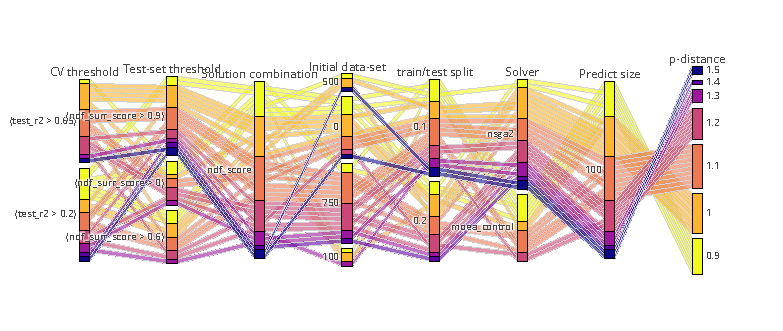
\includegraphics[width=\textwidth]{content/images/conf_zdt6_worst}
            \caption{40 worst configurations}
            \label{fig:conf_zdt6_worst}
        \end{subfigure} 
        % \hfill
        
        \begin{subfigure}{\textwidth}
            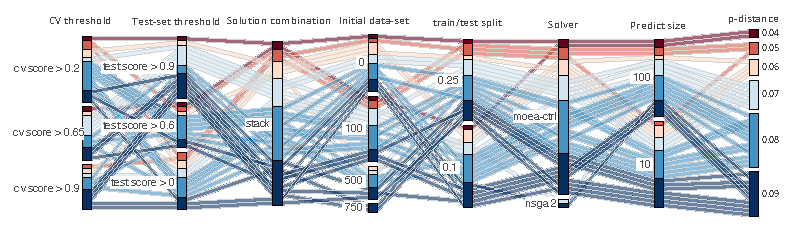
\includegraphics[width=\textwidth]{content/images/conf_zdt6_best}
            \caption{40 best configurations}
            \label{fig:conf_zdt6_best}
        \end{subfigure} 

        \caption[ZDT6: The selection from average result of best and worst configurations.]{ZDT6: The selection from average result of best and worst configurations.}
        \label{fig:conf_zdt6}    
    \end{figure}

    % === ZDT 6
    \begin{figure}
        \centering

        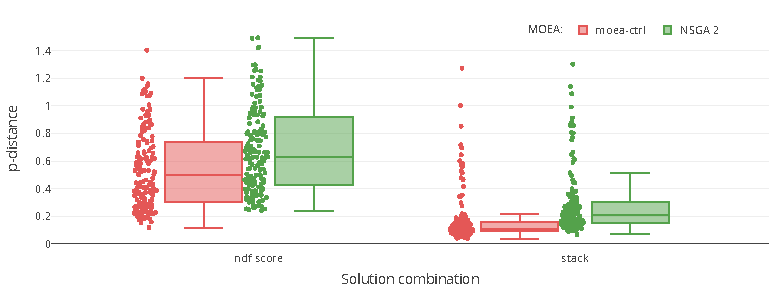
\includegraphics[width=0.8\textwidth]{content/images/conf_zdt6_solver}

        \caption[Correlation between the most influenceable parameters for the ZDT6]{Correlation between the most influenceable parameters for the ZDT6: solution combination strategy and optimization algorithm}
        \label{fig:conf_zdt6_sign}    
    \end{figure}


    % === -------------------------------------- ZDT 4
    \begin{figure}
        \centering
        \begin{subfigure}{\textwidth}
            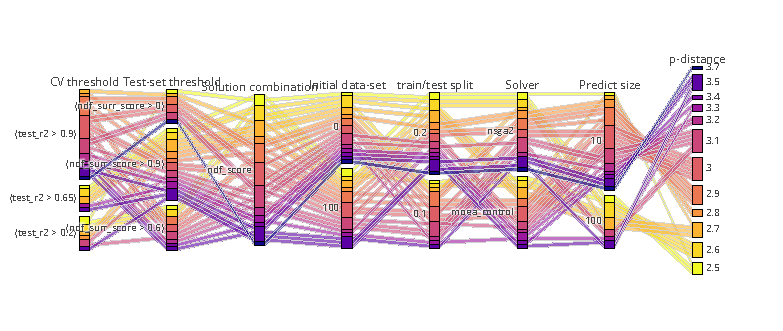
\includegraphics[width=\textwidth]{content/images/conf_zdt4_worst}
            \caption{ZDT4: worst configurations}
            \label{fig:conf_zdt4_worst}
        \end{subfigure} 
        \hfill
        
        \begin{subfigure}{\textwidth}
            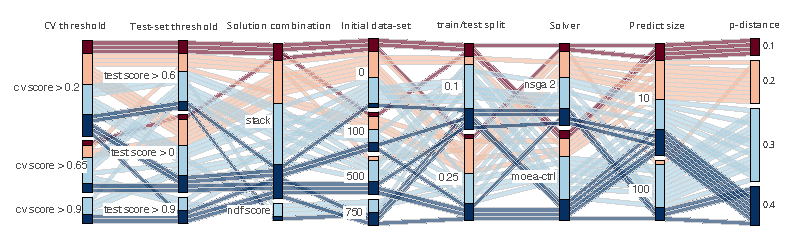
\includegraphics[width=\textwidth]{content/images/conf_zdt4_best}
            \caption{ZDT4: best configurations}
            \label{fig:conf_zdt4_best}
        \end{subfigure} 

        \caption[ZDT4: The selection from average result of best and worst configurations.]{ZDT4: The selection from average result of best and worst configurations.}
        \label{fig:conf_zdt4}    
    \end{figure}

    % === ZDT4
    \begin{figure}
        \centering
        \begin{subfigure}{\textwidth}
            \begin{subfigure}{0.45\textwidth}
                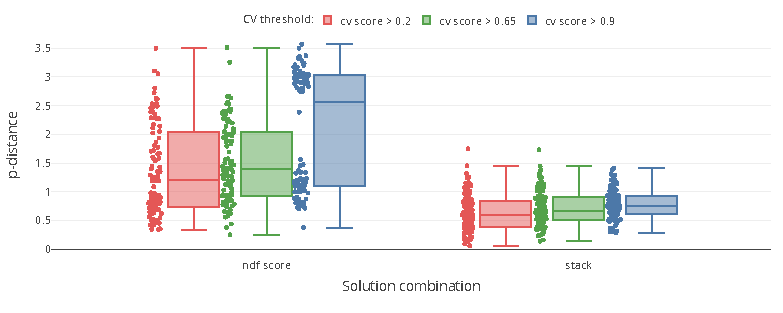
\includegraphics[width=\textwidth]{content/images/conf_zdt4_cv_score}
                \caption{An impact of the cross-validation's threshold}
                \label{fig:zdt4_pred_solver}
            \end{subfigure} 
            \begin{subfigure}{0.45\textwidth}
                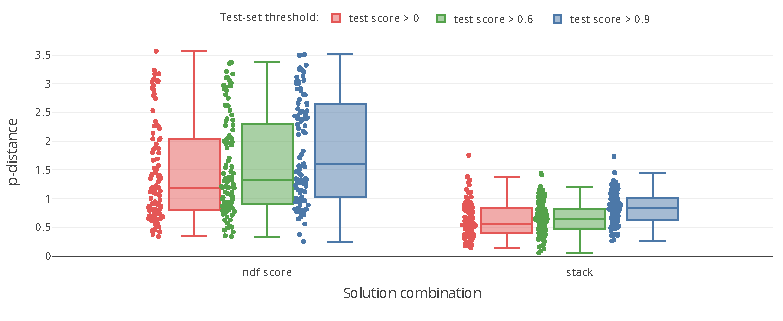
\includegraphics[width=\textwidth]{content/images/conf_zdt4_test_score}
                \caption{An impact of the test-set-validation's threshold}
                \label{fig:zdt4_comb_valid}
            \end{subfigure}
        \end{subfigure}


        \caption[Correlation between the most influenceable parameters for the ZDT4]{Correlation between the most influenceable parameters for the ZDT4} 
        \label{fig:conf_zdt4_sign}    
    \end{figure}

    % ====================================================== Start set for Hypermapper 2.0
    \subsection{Sampling plan size}
    Purpose of this experiment is to review the dependencies between the optimization result and the sampling plan size. The HyperMapper was selected as a foundation for analysis because it has a static implementation of the optimization algorithm with the surrogate model.

    The results are shown in the following figure \ref{fig:hmapper_start_set}. 
    For WFG1 and WFG4 problem, the criterion is the hypervolume and for ZDT4 and ZDT6 problem is the p-distance. Of all the results, the initial sampling plan is the least effects to the WFG6. Since this problem is unimodal and is described merely by fewer samples, other problems have a more complicated multimodal landscape that shown by unstable results. It is noticeable that the plan depends on the problem type. The optimization result may deteriorate which caused by increasing or decreasing the number of samples.

    \begin{figure}
        \centering
        \begin{subfigure}{\textwidth}
            \begin{subfigure}{0.45\textwidth}
                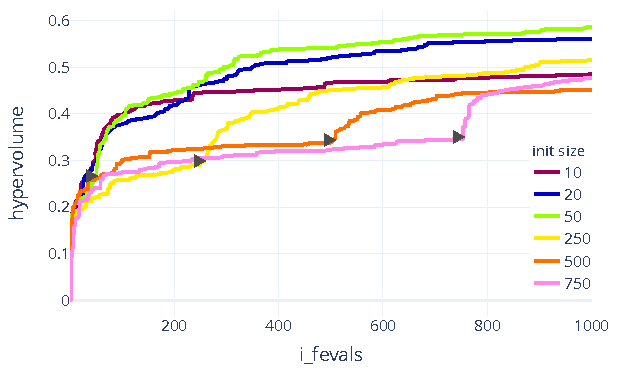
\includegraphics[width=\textwidth]{content/images/hypermapper_wfg1_start_set}
                \caption{WFG1}
                \label{fig:hmapper_wfg1_start_set}
            \end{subfigure}
            \begin{subfigure}{0.45\textwidth}
                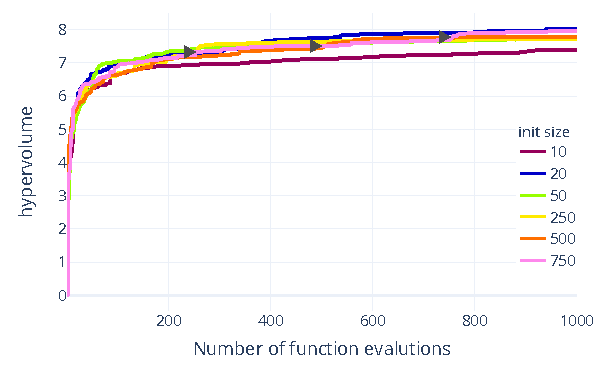
\includegraphics[width=\textwidth]{content/images/hypermapper_wfg4_start_set}
                \caption{WFG4}
                \label{fig:hmapper_wfg4_start_set}
            \end{subfigure}
        \end{subfigure} 
        \hfill

        
        \begin{subfigure}{\textwidth}
            \begin{subfigure}{0.45\textwidth}
                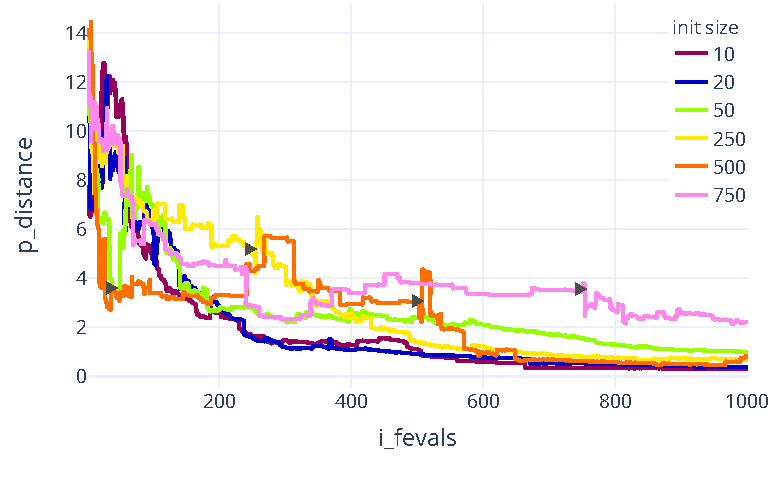
\includegraphics[width=\textwidth]{content/images/hypermapper_zdt4_start_set}
                \caption{ZDT4}
                \label{fig:hmapper_zdt4_start_set}
            \end{subfigure}
            \begin{subfigure}{0.45\textwidth}
                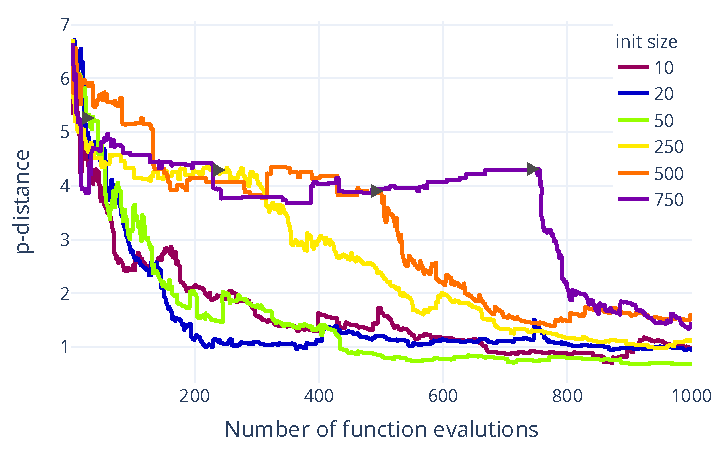
\includegraphics[width=\textwidth]{content/images/hypermapper_zdt6_start_set}
                \caption{ZDT6}
                \label{fig:hmapper_zdt6_start_set}
            \end{subfigure}
        \end{subfigure} 

        \caption[Influence of the initial sample plan for optimization with Hypermapper 2.0.]{Influence of the initial sample plan for optimization with Hypermapper 2.0.}
        \label{fig:hmapper_start_set}    
    \end{figure}



% --------------------------------------------------------------------------------------------
% ---------------------       Benchmark 3: Many-objective optimization, scaling
% --------------------------------------------------------------------------------------------
\section{Benchmark 3: Scalability of surrogate models. RQ1.1}
    Not only the type of the problem landscape but also its dimensions is an essential factor for picking the surrogate model. The advantage of a surrogate model might be lost when the number of optimization parameters or criteria are changed. The goal of this experiment is to find out the scalability of surrogate models. 


    The following surrogates were selected for verification:
    \begin{itemize}
        \item \emph{Gaussian Process Regressor} with kernel design from GPML\cite{RasmussenN10}. Gaussian process models are well known as commonly used in Bayesian optimization for a wide variety of problems. 
        \item MLPRegressor is a \emph{neural network} implementation from the \textit{sklearn} framework. Neural networks could automatically discover useful representations in high-dimensional data by learning multiple layers \cite{WilsonHSX16}. Because this model simultaneously extrapolates all objectives, we intuitively chose an architecture that consists of 5 layers and 100 neurons per layer.
        \item The surrogate portfolio is included of Gradient Boosting Regressor and \emph{SVR (RBF kernel)} as in the mentioned benchmark number 2. Also, a neural network with 5 cells and 50 neurons per layer was added. For the sake of the experiment, all models in the portfolio are composite and can be dynamically combined depending on the validation results. The surrogate portfolio is included of the Gradient Boosting Regressor and the SVR (RBF kernel). Also, a neural network with 5 layers and 50 neurons per layer was added. All models in the portfolio are composite and can be dynamically combined depending on the validation results.
    \end{itemize}

    For evaluation scalability property for the surrogate models, \emph{DTLZ2} problem was selected. It is unimodal problem with multiple global optima and concave geometry of the Pareto front. During the experiment, the number of optimization criteria changes with a constant number of parameters. For all cases, the experiment was repeated 5 times. The figure \ref{fig:scale_dtlz2} shows the three selected surrogate strategies with metrics of the average distance to the Pareto front (top line) and a time spent per complete an optimization iteration (bottom line). Note that the Gaussian model shows significantly better results relative to other approaches but only for the bi-objective problem. Increasing the criteria to 4, converging to a solution is only available for the neural network and portfolio. At the same time, the Gaussian model becomes incorrect and begins to increase the time required to build exponentially.
    
    There is also an open question as to which parameters to choose for the surrogate model. The suitability and quality of the surrogate are highly dependent on the parameters (number of layers, type of core). In turn, for the surrogate portfolio, the parameters determine how to build and select surrogate models. The same model but with different parameters, is evaluated in the portfolio as separate entities. It is a great advantage to apply a dynamic and scalable approach that can adapt to a specific problem. This is the answer to \hyperref[RQ1.1]{RQ1.1}.

    
    Hence, the necessary criterion for scaling surrogates is not just the choice of one model for all cases, but the dynamic combination of the strong properties of several models to achieve better results with limited resources.


    \begin{figure}
        \centering
        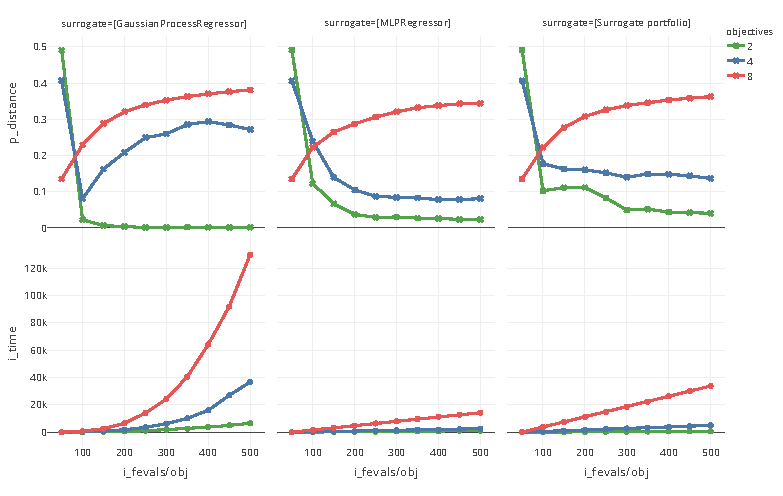
\includegraphics[width=\textwidth]{content/images/scale_dtlz2}
        \caption[Scaling example for the three variants of the surrogate on the DTLZ2.]{Scaling example for the three variants of the surrogate on the DTLZ2. Scaling example for the three variants of the surrogate on the DTLZ2  with the 9-dimensional objective space.}
        \label{fig:scale_dtlz2}    
    \end{figure}



    % 

    % Objectives: 1) detect iterative improvement, a convergence of the primary metric 2) time for evaluation

    % Usecases: GausianModel, GausianModel + Gradient, GausianModel + random forest, 

    % Scale: objectives - 2,4,8,10; params - 2,4,8,10

    % ! [ Hypermapper baseline; X - objectives Y - p-distance/time]




% --------------------------------------------------------------------------------------------
% ------------------------------------------------     Discussion 
% --------------------------------------------------------------------------------------------
\section{Discussion}

Up to now, most papers used the The quality of the results obtained with X was similar to the results obtained with Y, but with significantly fewer exactly evaluated solutions during the optimization process. 


% consume an inordinate amount of time.


The purpose of this work is to explore the possibility of using single-objective models for many-objective optimizations. To accomplish this goal, the composite model has been implemented. It is used to combine models into a portfolio and dynamically select them. Furthermore, the stepwise validation approach has been adapted to evaluate the usability of the surrogate model.

% Discussion

% non-separable
% or have a deceptive fitness landscape

% However, GAs, or at least some variants of them, are not 100'\%' ruled out.

% +’, ’−’ and ’≈’, which indicate that the result is significantly better, significantly worst and statistically similar to the result in the control column, respectively. 


% On the left side the learning curve of a naive Bayes classifier is shown for the digits dataset. Note that the training score and the cross-validation score are both not very good at the end. However, the shape of the curve can be found in more complex datasets very often: the training score is very high at the beginning and decreases and the cross-validation score is very low at the beginning and increases. On the right side we see the learning curve of an SVM with RBF kernel. We can see clearly that the training score is still around the maximum and the validation score could be increased with more training samples.
% https://scikit-learn.org/0.15/auto_examples/plot_learning_curve.html




% Compared to Auto-WEKA, this is much more data-efficient: in
% Auto-WEKA, evaluating the performance of an ensemble with 5 components requires the construction
% and evaluation of 5 models; in contrast, in auto-sklearn, ensembles come largely for free, and it is
% possible to mix and match models evaluated at arbitrary times during the optimization.


% This makes the archive gradually move towards the Pareto-front.
% 80% of the computing-time is spent in the area close to the Pareto front.


% We would like to prove that the use of hierarchical surrogates has a higher probability to find the optimum of the optimization problem in Eq. (4) ref[Evolutionary optimization with hierarchical surrogates]


% Test problems ZDT1, ZDT2, and ZDT3 show a different trend in function evaluations as compared to OSY.


% In contrast to PR, ANN, RBF, GP, Ranking SVM is invariant to

% The measurements were performed on an Intel Core i7-8700CPU machine with 64G of memory using Fedora Server 29.












    % The first benchmark presented a subset of the problems listed in Table \ref{bench_problems}. They have a wide range of properties which should give a notion of how the optimization strategy works.
    % % ==== multi-objective test problems
    % \begin{table}[]
    %     \centering
    %     \resizebox{\textwidth}{!}{%
    %         \begin{tabular}{@{}cccccc@{}}
    %         \toprule
    %         \multirow{2}{*}{\textbf{Problem}} &
    %         \multirow{2}{*}{\textbf{Objective}} &
    %         \multirow{2}{*}{\textbf{Modality}} &
    %         \multirow{2}{*}{\textbf{Geometry}} &
    %         \multicolumn{2}{c}{\textbf{Landscape}} \\ \cmidrule(l){5-6}
    %                     &                 &                      &               & \textbf{Bias}    & \textbf{\begin{tabular}[c]{@{}c@{}}Many-to-one \\ mappings\end{tabular}} \\ \midrule
    %         \textbf{ZDT4}  & bi-objective    & unimodal, multimodal & convex        & -                & -                                                                        \\
    %         \textbf{ZDT6}  & bi-objective    & multimodal           & concave       & +                & +                                                                        \\
    %         \textbf{DTLZ4} & multi-objective & unimodal             & concave       & +                & +                                                                        \\
    %         \textbf{WFG1}  & multi-objective & unimodal             & convex, mixed & polynomial, flat & +                                                                        \\
    %         \textbf{WFG4}  & multi-objective & multimodal           & concave       & -                & +                                                                       \\ \bottomrule
    %         \end{tabular}%
    %     }
    %     \caption{Selected multi-objective test problems}
    %     \label{bench_problems}
    % \end{table}